\documentclass[12pt]{article}
\usepackage{geometry} 
\usepackage{amsmath,amsthm,amssymb,scrextend}
\usepackage{fancyhdr}
\setlength{\headheight}{14.5pt}
\addtolength{\topmargin}{-2.5pt}
\pagestyle{fancy}

\newcommand{\cont}{\subseteq}
\usepackage{tikz}
\usepackage{pgfplots}
\usepackage{amsmath}
\usepackage[mathscr]{euscript}
\let\euscr\mathscr\let\mathscr\relax% just so we can load this and rsfs
\usepackage[scr]{rsfso}
\usepackage{amsthm}
\usepackage{amssymb}
\usepackage{multicol}
\usepackage[colorlinks=true, pdfstartview=FitV, linkcolor=blue,
citecolor=blue, urlcolor=blue]{hyperref}
\usepackage{graphicx}
\usepackage{float}
\usepackage{listings}
\usepackage{color}
\usepackage{xcolor}
\definecolor{codegreen}{rgb}{0,0.6,0}
\definecolor{codegray}{rgb}{0.5,0.5,0.5}
\definecolor{codepurple}{rgb}{0.58,0,0.82}
\lstset{
			backgroundcolor=\color{red!50!green!50!blue!50!white!20},
			breaklines = true,
			tabsize=2,
			commentstyle=\color{codegreen},
			keywordstyle=\color{magenta},
			numberstyle=\tiny\color{codegray},
			stringstyle=\color{codepurple},
	    }
\DeclareMathOperator{\arcsec}{arcsec}
\DeclareMathOperator{\arccot}{arccot}
\DeclareMathOperator{\arccsc}{arccsc}
\newcommand{\ddx}{\frac{d}{dx}}
\newcommand{\dfdx}{\frac{df}{dx}}
\newcommand{\ddxp}[1]{\frac{d}{dx}\left(#1 \right)}
\newcommand{\dydx}{\frac{dy}{dx}}
\newcommand{\intx}[1]{\int#1 \, dx}
\newcommand{\intt}[1]{\int#1 \, dt}
\newcommand{\defint}[3]{\int_{#1}^{#2} #3 \, dx}
\newcommand{\imp}{\Rightarrow}
\newcommand{\un}{\cup}
\newcommand{\inter}{\cap}
\newcommand{\ps}{\mathscr{P}}
\newcommand{\set}[1]{\left\{ #1 \right\}}
\newtheorem*{sol}{Solution}
\newtheorem*{claim}{Claim}
\newtheorem{problem}{Problem}
\pgfplotsset{compat=1.17}
\begin{document}
 
% Don't change the above session

\lhead{22 AI-BD/problem 6.}
\chead{107205008, 109102057}
\rhead{\today}
 
% \maketitle
\section*{problem 1.}
    \begin{lstlisting}[language = Matlab]
        data = readtable('bank.csv');
        trainX = table2array(data(1:2000, ["age", "balance"]));
        trainY = ones(2000,1);
        for i =1:2000
            if string(data{i,"y"})=="no"
                trainY(i,1)=-1;
            else 
                trainY(i,1)=1;
            end
        end
        [train_num,dim]=size(trainX);
        w=ones(1,dim+1);
        h=zeros(train_num,1);
        x=[ones(train_num,1) trainX];
        while 1
            for i =1:20
                h(i,:)=sign(x(i,:)*w');
                if h(i,:)~=trainY(i,:) 
                w=w+trainY(i,:)*x(i,:); 
                w
                end
            end
            if h==trainY  
                break
            end
        end
        scatter(trainX(:, 1), trainX(:,2), [], trainY)
        colormap([1 0 0; 0 0 1])
        saveas(gcf,'scatter.png')
    \end{lstlisting}
$\bullet$ After we revise the code, because PLA learning method is linearly separable, we 
can't use only 2 explanatory variables to calssify the data.\\\\
$\bullet$ We found that in the $while$ loop, if we set $i = 20$, the output will be infinity loop. Based on this solution, we draw a scatter plot of the data.

\begin{figure}[H]
    \centering
    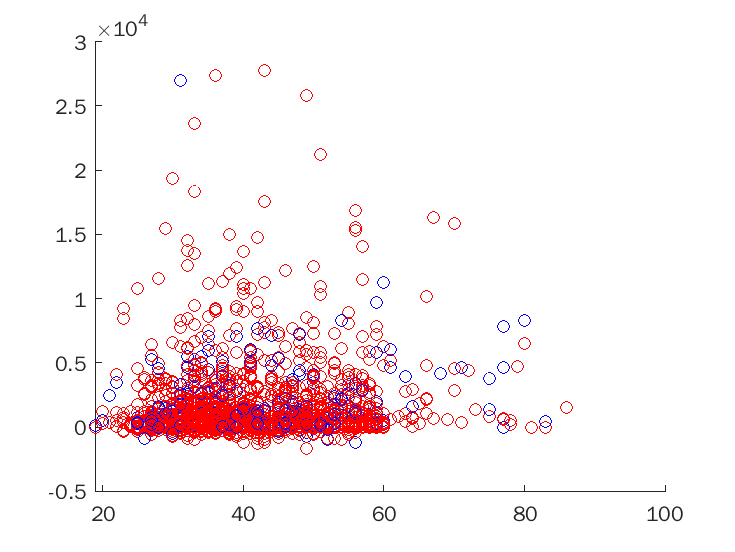
\includegraphics[width = 0.7\textwidth]{scatter.png}
    \caption{scatter plot of first 2000 data of bank}
\end{figure}
$\bullet$ the blue circle denotes `Yes'
\newline
\hspace*{6.2mm}$\bullet$ the red circle denotes `No'

    
\end{document}
